\chapter{Introduction} \label{chap:introduction}

The use of modern technologies in the home opens up new possibilities for managing the user's time and efficient energy management. The smart home responds to the user's needs and uses automatic control to increase the comfort of living in the home. The smart home centre is a complex system with various separate modules which collects locally measured data. Based on this data and active interventions from the user, it automates operation in the home. The features of a smart home include the ability for the user to interact with the system easily. This is often addressed through a website or voice interaction. This project focuses on one aspect of the smart home - enabling the user to built modules and control them by voice.


The voice-enabled modules help the user control the smart home more easily, and the entire solution's comfort is increased. Thus, the user can minimize the energy expended on operating a smart home. The user simply says his command or question and gets answers in a voice with the system's action, so the user does not have to go anywhere or even interrupt his work.


The work aims are to build a modular functional system with voice-enabled modules for the smart home, which fulfil specific real applications. The project consists of several development boards connected to several lights and sensors measuring different physical quantities. These control and analytical components are connected to a central modular functional system. An essential part of this thesis is creating voice-enabled modules implemented in the central control system and their connection to a virtual assistant. By using this virtual assistant, the user can control the function modules by voice. The entire project is accessible to the user via a web interface, which clearly provides all available information.

\section{State of the Art} \label{sec:state_of_the_art}

% /** General

The most famous intelligent personal assistants include Alexa, Siri, Google Assistant. These virtual assistants work on a very similar principle as follows. The assistant constantly listens to its surroundings to see if a wake-up word has been spoken. Assistant process this analysis of wake-up word on its hardware. After saying the wake-up word, the assistant starts recording a sound and analyzes simultaneously if no one is talking anymore. This recorded sound then assistant send to the appropriate servers for processing. The server handles the relevant device or service according to the processed user command and sends a synthesized audio response back to the assistant.

Siri's first assistant was created by Apple in 2010 and shortly followed by Cortana by Microsoft in 2013 and Alexa by Amazon in 2014. The growing power of computers and advancing cloud technology allows scientists and software engineers to train voice assistants more easily. Over time, voice assistants can respond to the user more naturally and give the user the feeling of talking to a person. 

In addition to these tasks, the user can connect the voice assistant to web services (see \cref{fig:voice_assistant_connecrtion_schema}) like Tasker, IFTTT and other features (often called "skills") developed by third-party developers. By these additions, the user adds a new palette of commands such as automating social media posts, ordering a usual drink from a local Starbucks or summoning an Uber or Lyft using connected account data.

\begin{figure}[H]
    \centering
    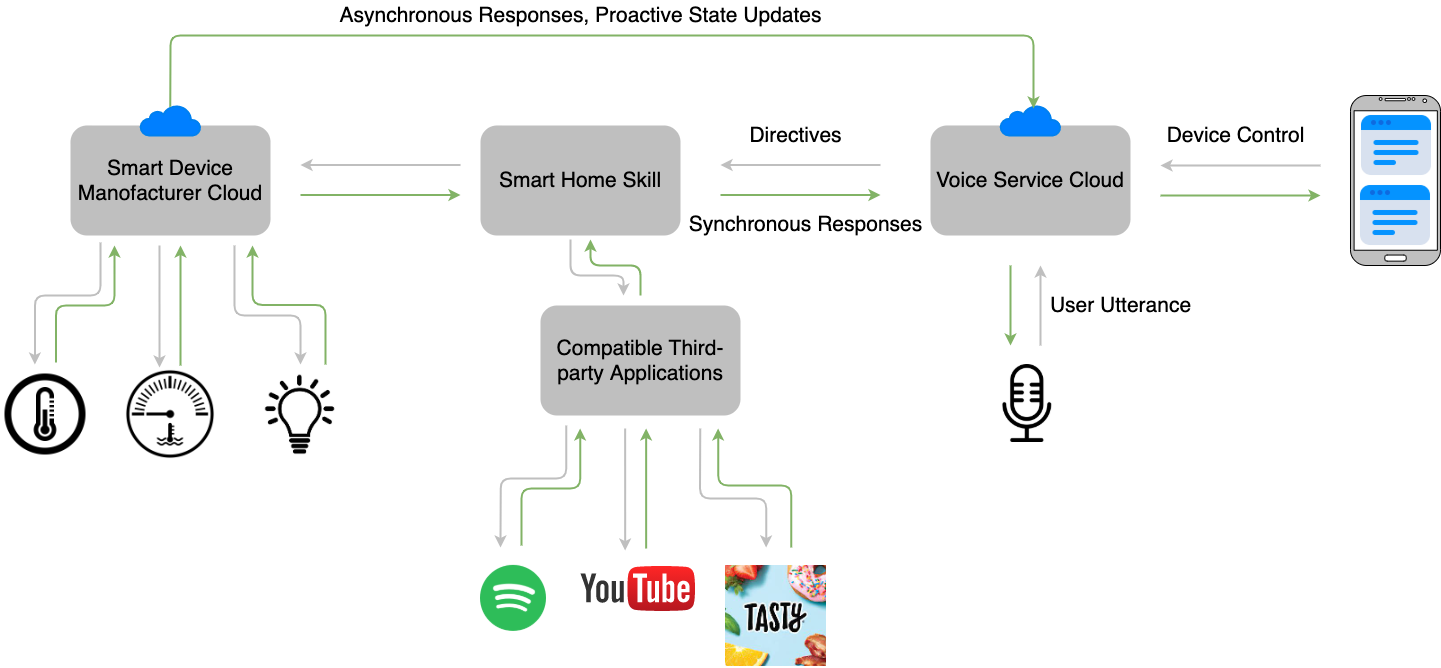
\includegraphics[width=\textwidth]{img/voice_assistant_to_server_connection.png}
    \caption{Connection schema of voice assistant service \citep{voice_assistant_service}}
    \label{fig:voice_assistant_connecrtion_schema}
\end{figure}
\newpage
Although each currently available voice assistant has unique features, they share some similarities and are able to perform the following basic tasks \citep{voice_assistants_general_hoy_2018}: 

\begin{itemize}
    \item send and read text messages, make phone calls, and send and read email messages; 
    \item answer basic informational queries (“What time is it? What’s the weather forecast? How many ounces are in a cup?”); 
    \item set timers, alarms, and calendar entries;
    \item set reminders, make lists, and do basic math calculations;
    \item control media playback from connected services such as Amazon, Google Play, iTunes, Pandora, Netflix, and Spotify; 
    \item control  Internet-of-Things-enabled  devices  such  as  thermostats,  lights, alarms, and locks; and 
    \item tell jokes and stories. 
\end{itemize}

\subsection{Comparison of SotA Assistant}

Because each company develop its voice assistant independently and protect its knowledge, these assistants are quite different despite their common ground. Figure \cref{fig:voice_assistant_comparison} determine the most capable assistant by asking 800 questions that consist of categories like \citep{voice_assistant_comparison_munster_2019}:

\begin{itemize}
    \item Local – Where is the nearest coffee shop?
    \item Commerce – Order me more paper towels.
    \item Navigation – How do I get to Uptown on the bus?
    \item Information – Who do the Twins play tonight?
    \item Command – Remind me to call Jerome at 2 pm today.
\end{itemize}

Google Assistant has answered 93\% correctly and has understood all 800 questions correctly. Siri has been next, has answered 83\% correctly and has misunderstood only two questions. Alexa has answered 80\% correctly and has misunderstood only one. According to the data shown in \cref{fig:voice_assistant_comparison}, Google Assistant has better results overall but lacks in the command category. Amazon Alexa has excellent results only in the information category, where it climbs just below the results of Google Assistant. Siri is brilliant in the command category for such functions as a calling, sending SMS or playing music.

\begin{figure}[H]
    \centering
    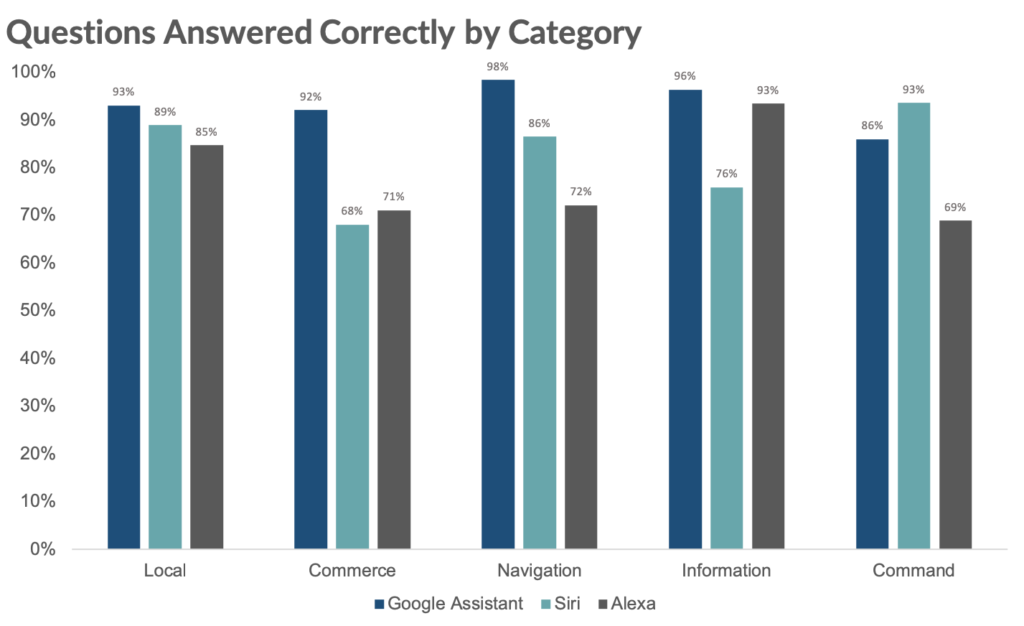
\includegraphics[width=\textwidth]{img/voice_assistant_comparison.png}
    \caption{Voice assistant comparison by types of questions \citep{voice_assistant_comparison_munster_2019}}
    \label{fig:voice_assistant_comparison}
\end{figure}

If several users occupy the room, each voice assistant has its way of handling this situation. For example, Amazon Alexa and Google Assistant create multiple voice profiles, which allows the user to train the assistant to recognize his voice specifically and therefore offer different data and use separate accounts for services. This is a very complex task, and no one can cope with it at the desired level.

% assistants comparison
% https://www.researchgate.net/publication/337407222_User_Experience_Comparison_of_Intelligent_Personal_Assistants_Alexa_Google_Assistant_Siri_and_Cortana

% https://www.researchgate.net/publication/329624889_Using_intelligent_personal_assistants_to_assist_the_elderlies_An_evaluation_of_Amazon_Alexa_Google_Assistant_Microsoft_Cortana_and_Apple_Siri

\section{The market gap}
% -dialogue in czech
% -general backend / Modularity
% -openSource (own end2end project)
% -tools like DB, webserver, mqtt

This project responds to the gap in the market given by the following factors:

\begin{itemize}
    \item \textit{Dialogue in the Czech Language}:
    The Czech language is a significant gap in the market in the virtual assistant sector. This gap in the market is caused by the number of people who speak this language. Because the development of this technology is still not complete and costs much money, this low demand market is not interesting for large institutions building virtual assistants.

    Another reason why large technological institutions are not interested in developing virtual assistants for Czech-speaking people is the grammatical and verbal complexity of the Czech language. The Czech language is much more complicated than English. It has many declension, gradation of adjectives, words depending on the sentence and different conjugation.
\newpage
    So far, known activities in this market are that Siri does not speak in the Czech language, and there are no publicly known prospects that she would be able to do shortly. Google Assistant does not offer to speak in the Czech language either, but it has TTS and ASR support in the Czech language.
    \item \textit{Modularity of Virtual Assistants}:
    Although this problem has been largely resolved, as described in \cref{sec:state_of_the_art}, the user is still widely limited and cannot ask the virtual assistant anything he would like. However, technology companies are working hard to resolve this issue to become more and more an issue of the past overtime.
    \item \textit{Open-source Projects}:
    There are several open-source projects on the market, such as openHAB, Home Assistant and OpenMotics. However, setting them up is complicated and requires much technical knowledge. These projects already have a relatively large community and have many packages and modules to connect.
    % This project is open-source, which means that customers can participate in the development as with the end-to-end project. This aspect is vital because the people who use this product know best where the weakest point of the project is. Furthermore, since the usability of this project depends on the number of modules (described in \cref{chap:modules}), these things can be shared between users and thus increase the user experience.
    % \item \textit{Availability of Tools}:
    % There are already many tools on the Internet that aim for the Internet of Things. These tools include, for example, MQTT, Arduino, Node-RED, ESP development board, MongoDB. These tools are open-source and resolving a wide range of issues, such as communication, which would not be easy to solve from scratch. These tools make development in the Internet of Things field much more effortless and secure.
\end{itemize}

% \subsection{Dialogue in the Czech Language}
% The Czech language is a significant gap in the market in the virtual assistant sector. This gap in the market is caused by the number of people who speak this language. Because the development of this technology is still not complete and costs much money, this low demand market is not interesting for large institutions building virtual assistants.

% Another reason why large technological institutions are not interested in developing virtual assistants for Czech-speaking people is the grammatical and verbal complexity of the Czech language. The Czech language is much more complicated than English. It has many declension, gradation of adjectives, words depending on the sentence and different conjugation.

% \subsection{Modularity of Virtual Assistants}

% Although this problem has been largely resolved, as described in \cref{sec:state_of_the_art}, the user is still widely limited and cannot ask the virtual assistant anything he would like. However, technology companies are working hard to resolve this issue to become more and more an issue of the past overtime.

% \subsection{Open-source Projects}

% This project is open-source, which means that customers can participate in the development as with the end-to-end project. This aspect is vital because the people who use this product know best where the weakest point of the project is. Furthermore, since the usability of this project depends on the number of modules (described in \cref{chap:modules}), these things can be shared between users and thus increase the user experience.

% \subsection{Availability of Tools}
% % \cref{chap:backend}
% There are already many tools on the Internet that aim for the Internet of Things. These tools include, for example, MQTT, Arduino, Node-RED, ESP development board, MongoDB. These tools are open-source and resolving a wide range of issues, such as communication, which would not be easy to solve from scratch. These tools make development in the Internet of Things field much more effortless and secure.



\section{Thesis Objectives} \label{sec:thesis_objectives}

% Až budeš psát thesis objectives, navrhuji držet se následujících bodů (souvisí s oficiálním zadáním práce):

% Hlavní cíl: navržení obecného komunikačního rozhraní pro hlasově ovládané moduly chytré domácnosti

% Dílčí cíle:
% 1/ otestování vybraných modulů pro využití v projektu
% 2/ fyzická realizace hardwarově závislých modulů
% 3/ řešení rozhraní mezi uživatelem a moduly (backend)
% 4/ přidání hlasové interakce
% 5/ dle časů a možností obohacení o další moduly


% Učeš to podle svého mínění, ale držel bych podobnou kostru.

The objectives of this study are:

\begin{enumerate}
    \item to test selected modules for use in the project;
    \item to implement hardware-dependent modules physically;
    \item to design an interface for communication between the user and selected modules;
    \item to add an interface for voice interaction;
    \item to enrich the project with other modules according to the time possibilities.
\end{enumerate}

\section{Thesis Outline} \label{sec:thesis_outline}

This thesis consists of 7 chapters following the standard skeleton of scientific publications.

Chapter 1 describes the current trends of virtual assistants and compares them. It then explains the gap in the market that this project meets and its advantages over other solutions.

Chapter 2 lists the general methods used in automatic speech recognition and automatic speech synthesis fields and briefly describes them. Furthermore, the chapter briefly describes the functions and architecture of the SpeechCloud used as ASR and TTS interface for the project.
\newpage
Chapter 3 discusses in more detail the architecture used for the system running on the server. The chapter further specifies the type of database used and its benefits for the project. Furthermore, three used communication protocols and their benefits for the project are listed here. At the end of this chapter, we describe the three controllers users use to communicate with the modules and how they work or when they are used.

Chapter 4 lists five created modules. The chapter describes its functions, a code diagram of the functions, the voice commands triggering the functions (a detailed list of the voice commands is then given in appendix A2), used electrical circuits and message structures in more detail for each module.

Chapter 5 shows and describes the created web controller. The chapter defines the used libraries, frameworks and server address. It also describes all the available features and how the data on the page changes over time.

Chapter 6 comes with the discussion about the results. It also contains a comparison of the developed system to the presented state-of-the-art technology from section 1.1. Then, ideas for future work are suggested. The study is concluded in Chapter 7.

Appendix A1 contains a figure of algorithm diagram of the ESP that did not fit the main text but can still be interesting for some readers. As mentioned above, appendix A2 gives a detailed list of voice commands for each module described in chapter 4.